\documentclass[11pt]{article}
\usepackage{amsmath, amssymb, physics, mathtools, bm}
\usepackage{tikz, pgfplots}
\pgfplotsset{compat=1.18}
\usepackage[margin=2.3cm]{geometry}
\usepackage{siunitx, booktabs, hyperref}
\usepackage{braket}

\newcommand{\D}{\mathrm{D}}
\newcommand{\de}{\mathrm{d}}
\newcommand{\pd}[2]{\frac{\partial #1}{\partial #2}}
\newcommand{\pdd}[2]{\frac{\partial^{2} #1}{\partial #2^{2}}}
\newcommand{\Lap}{\nabla^{2}}

\title{B6 Condensed-Matter Physics --- Model Solutions, 2020}
\author{}
\date{}

\begin{document}
\maketitle

%==================================================================
\section*{Question 1 --- FCC structure factor and Si powder diffraction}

\textbf{Problem.} (a) Derive the FCC selection rule and show the per-basis-atom contribution is $4f\,e^{2\pi i(hx+ky+lz)}$. (b) Show $|S_{\{hkl\}}|^2 = 32 f_\text{Si}^2(1+\cos(n\pi/2))$ for diamond Si and identify $n$. (c) Give $d_{hkl}$ and powder multiplicities for $(002)$, $(111)$. (d) Complete a powder-pattern table for neutrons at $\lambda = \SI{0.1542}{nm}$. (e) X-ray vs.\ neutron intensity ratio as a function of $2\theta$.

\subsection*{(a) FCC extinction rule}

Four FCC atoms at $\bm r + (0,0,0)$, $\bm r+(\tfrac12,\tfrac12,0)$, $\bm r+(\tfrac12,0,\tfrac12)$, $\bm r+(0,\tfrac12,\tfrac12)$ with $\bm r = (x,y,z)$. Sum the plane-wave phases:
\[
S_\text{FCC}(hkl) = f\,e^{2\pi i(hx+ky+lz)}\bigl[1 + e^{i\pi(h+k)} + e^{i\pi(h+l)} + e^{i\pi(k+l)}\bigr].
\]
Reduce each exponential using $e^{i\pi m} = (-1)^m$:
\[
e^{i\pi(h+k)} = (-1)^{h+k},\quad e^{i\pi(h+l)} = (-1)^{h+l},\quad e^{i\pi(k+l)} = (-1)^{k+l}.
\]
All $h,k,l$ same parity (all even / all odd) makes every index sum even:
\[
1 + 1 + 1 + 1 = 4.
\]
Mixed parity: exactly two of the three sums $(h+k,h+l,k+l)$ are odd:
\[
1 + 1 - 1 - 1 = 0.
\]
Therefore the bracket equals $4$ when $h,k,l$ are all even or all odd, and $0$ otherwise:
\begin{equation}
\boxed{\;S_\text{FCC}(hkl) = 4f\,e^{2\pi i(hx+ky+lz)}\quad\text{(non-extinct: }h,k,l\text{ all even or all odd)}.\;}
\label{eq:fcc-factor}
\end{equation}

\subsection*{(b) Diamond-Si structure factor}

Two basis atoms at $(0,0,0)$ and $(\tfrac34,\tfrac14,\tfrac34)$, each carrying the FCC factor \eqref{eq:fcc-factor}:
\[
S_{\{hkl\}} = 4 f_\text{Si}\bigl[1 + e^{2\pi i(3h/4 + k/4 + 3l/4)}\bigr].
\]
Collect the exponent over a common denominator $4$:
\[
2\pi\!\left(\tfrac{3h}{4} + \tfrac{k}{4} + \tfrac{3l}{4}\right) = \frac{2\pi(3h+k+3l)}{4} = \frac{\pi}{2}(3h+k+3l).
\]
Define $n = 3h+k+3l$ (integer):
\[
S_{\{hkl\}} = 4 f_\text{Si}\bigl[1 + e^{i n\pi/2}\bigr].
\]
Take modulus squared with $|1+e^{i\phi}|^2 = 2(1+\cos\phi)$:
\[
|S_{\{hkl\}}|^2 = 16 f_\text{Si}^2 \cdot 2\!\left(1+\cos\frac{n\pi}{2}\right).
\]
Combine the constants:
\begin{equation}
\boxed{\;|S_{\{hkl\}}|^2 = 32 f_\text{Si}^2\!\left(1+\cos\frac{n\pi}{2}\right),\qquad n = 3h+k+3l.\;}
\label{eq:si-S2}
\end{equation}

\subsection*{(c) Plane spacing and multiplicities}

Cubic lattice:
\[
\boxed{\;d_{(hkl)} = \frac{a}{\sqrt{h^2+k^2+l^2}}.\;}
\]
\textbf{$\bm{m_{(002)}}$:} $\{200\}$-type permutations with one non-zero index $\pm 2$:
\[
(\pm 2,0,0),(0,\pm 2,0),(0,0,\pm 2)\implies m_{(002)} = 6.
\]
\textbf{$\bm{m_{(111)}}$:} all sign combinations of $(1,1,1)$:
\[
2\times 2\times 2 = 8\implies m_{(111)} = 8.
\]

\subsection*{(d) Neutron powder table}

Bragg's law: $\sin\theta = \lambda/(2 d_{hkl})$, $\lambda = \SI{0.1542}{nm}$, $a = \SI{0.543}{nm}$.

For each peak compute $n=3h+k+3l$, $|S|^2/f_\text{Si}^2$ from \eqref{eq:si-S2}, multiplicity $m$:
\begin{itemize}
\item $(111)$: $n=7$, $\cos(7\pi/2)=0$, $|S|^2=32 f^2$; $m=8$.
\item $(200)$: $n=6$, $\cos(3\pi)=-1$, $|S|^2=0$; $m=6$ (extinct).
\item $(220)$: $n=8$, $\cos(4\pi)=1$, $|S|^2=64 f^2$; $m=12$.
\item $(311)$: $n=13$, $\cos(13\pi/2)=0$, $|S|^2=32 f^2$; $m=24$.
\item $(400)$: $n=12$, $\cos(6\pi)=1$, $|S|^2=64 f^2$; $m=6$.
\end{itemize}

Compute $d_{hkl} = a/\sqrt{h^2+k^2+l^2}$:
\[
d_{111} = \frac{0.543}{\sqrt{3}} = \SI{0.3135}{nm},\quad d_{200} = \frac{0.543}{2} = \SI{0.2715}{nm},\quad d_{220} = \frac{0.543}{\sqrt{8}} = \SI{0.1920}{nm}.
\]
\[
d_{311} = \frac{0.543}{\sqrt{11}} = \SI{0.1637}{nm},\qquad d_{400} = \frac{0.543}{4} = \SI{0.1358}{nm}.
\]
Then $2\theta = 2\arcsin[\lambda/(2d)]$. For $(111)$:
\[
\sin\theta_{111} = \frac{0.1542}{2\cdot 0.3135} = 0.2460 \implies 2\theta_{111} = 2\arcsin(0.2460) = \SI{28.47}{\degree}.
\]
The remaining peaks follow identically; tabulated below:

\begin{center}
\begin{tabular}{cccccrr}
\toprule
peak & $\{hkl\}$ & $d_{\{hkl\}}/\si{nm}$ & $2\theta_{\{hkl\}}/\si{\degree}$ & $m$ & $I_\text{calc}/f_\text{Si}^2$ & $I_\text{meas}$ \\
\midrule
a & 111 & 0.3135 & 28.47 & 8  & 256  & 1000 \\
b & 200 & 0.2715 & 33.01 & 6  & 0    & 0    \\
c & 220 & 0.1920 & 47.40 & 12 & 768  & 2755 \\
d & 311 & 0.1637 & 56.18 & 24 & 768  & 2619 \\
e & 400 & 0.1358 & 69.20 & 6  & 384  & 1203 \\
\bottomrule
\end{tabular}
\end{center}

Ratio $I_\text{meas}/I_\text{calc}$ (should be a single constant $\propto b_\text{Si}^2$):
\[
\text{(a)}\,3.91,\quad\text{(c)}\,3.59,\quad\text{(d)}\,3.41,\quad\text{(e)}\,3.13.
\]
Ratios decrease with $2\theta$: \textbf{Debye--Waller damping} $e^{-2W}$ with $W\propto \sin^2\theta/\lambda^2$ suppresses high-angle peaks. Otherwise the agreement (constancy of the ratio) is good.

\subsection*{(e) X-rays vs.\ neutrons}

\textbf{(i)} Replace the neutron Fermi length $b_\text{Si}$ by the X-ray atomic form factor $f_\text{Si}(Q)$, which is $Q$-dependent (Fourier transform of the electron density), so $|S|^2 = 32\, f_\text{Si}^2(Q)\,(1+\cos(n\pi/2))$.

\textbf{(ii)} $f_\text{Si}(Q)$ falls monotonically with $Q$ (and thus with $2\theta$), while $b_\text{Si}$ is $Q$-independent (point nuclear scatterer). Hence
\[
\boxed{\;\frac{I_X}{I_n}\propto\frac{f_\text{Si}^2(2\theta)}{b_\text{Si}^2}\quad\text{decreases monotonically with }2\theta_{hkl}.\;}
\]

%==================================================================
\section*{Question 2 --- 2D Debye theory and graphene}

\textbf{Problem.} (a) Derive 2D Debye wavevector. (b) Find $\omega_D$, $T_D$, $g(\omega)$ for linear ($\omega=ck$, two polarisations) and quadratic ($\omega=Dk^2$, one polarisation) modes. (c) Low-$T$ molar specific heat in form $R\alpha(T/T_D)^\beta$. (d) Apply to graphene: $c_v = R(c_1 T + c_2 T^2)$, find $c_1, c_2$. (e) Compare to room-$T$ data.

\subsection*{(a) 2D Debye wavevector}

One atom per cell in 2D has $2N$ vibrational degrees of freedom, hence $N$ modes per polarisation. Equate the $k$-space disc area times the 2D mode density to the mode count:
\[
\frac{A}{(2\pi)^2}\,\pi k_D^2 = N.
\]
Rearrange for $k_D^2$:
\[
k_D^2 = \frac{4\pi^2 N}{\pi A} = \frac{4\pi N}{A}.
\]
Use $n = N/A$:
\[
k_D^2 = 4\pi n.
\]
Take square root:
\begin{equation}
\boxed{\;k_D = 2\sqrt{\pi n},\qquad a = 2\sqrt{\pi}.\;}
\label{eq:kD2D}
\end{equation}

\subsection*{(b) $\omega_D$, $T_D$, $g(\omega)$}

\textbf{(i) Linear mode $\omega=ck$, two polarisations.}

Cut-off:
\[
\omega_D = c\,k_D = 2c\sqrt{\pi n}.
\]
Debye temperature:
\[
\boxed{\;k_B T_D = \hbar\omega_D = 2\hbar c\sqrt{\pi n}.\;}
\]
DOS per polarisation per unit area from a 2D shell of radius $k$:
\[
g_1(\omega)\,\de\omega = \frac{1}{(2\pi)^2}\cdot 2\pi k\,\de k = \frac{k}{2\pi}\,\de k.
\]
Substitute $k = \omega/c$, $\de k = \de\omega/c$:
\[
g_1(\omega)\,\de\omega = \frac{1}{2\pi}\cdot\frac{\omega}{c}\cdot\frac{\de\omega}{c}.
\]
Divide both sides by $\de\omega$:
\[
g_1(\omega) = \frac{\omega}{2\pi c^2}.
\]
Multiply by two degenerate polarisations:
\[
g(\omega) = 2 g_1(\omega) = \frac{\omega}{\pi c^2}.
\]
Read off:
\begin{equation}
\boxed{\;g(\omega) = \gamma\,\omega,\qquad \gamma = \frac{1}{\pi c^2}\quad\text{(per unit area)}.\;}
\label{eq:gw-linear}
\end{equation}

\textbf{(ii) Quadratic mode $\omega=Dk^2$, one polarisation.}

Cut-off:
\[
\omega_D = D\,k_D^2 = 4\pi D n.
\]
Debye temperature:
\[
\boxed{\;k_B T_D = \hbar\omega_D = 4\pi\hbar D n.\;}
\]
DOS per unit area: invert $\omega = Dk^2$:
\[
k = \sqrt{\omega/D},\qquad \de k = \frac{\de\omega}{2\sqrt{D\omega}}.
\]
Single polarisation contribution:
\[
g(\omega)\,\de\omega = \frac{k}{2\pi}\,\de k = \frac{1}{2\pi}\,\sqrt{\frac{\omega}{D}}\cdot\frac{\de\omega}{2\sqrt{D\omega}}.
\]
Cancel $\sqrt{\omega}$ in numerator and denominator:
\[
g(\omega)\,\de\omega = \frac{1}{4\pi D}\,\de\omega.
\]
Divide both sides by $\de\omega$:
\begin{equation}
\boxed{\;g(\omega) = \gamma',\qquad \gamma' = \frac{1}{4\pi D}\quad\text{(per unit area)}.\;}
\label{eq:gw-quad}
\end{equation}

\subsection*{(c) Low-$T$ specific heat}

Energy per unit area at temperature $T$:
\[
u(T) = \int_0^{\omega_D}\!\!g(\omega)\,\frac{\hbar\omega}{e^{\beta\hbar\omega}-1}\,\de\omega.
\]
Low-$T$ limit: extend upper limit to $\infty$.

\textbf{Case (i):} substitute \eqref{eq:gw-linear}:
\[
u = \int_0^\infty\!\frac{1}{\pi c^2}\,\omega\,\frac{\hbar\omega}{e^{\beta\hbar\omega}-1}\,\de\omega = \frac{\hbar}{\pi c^2}\int_0^\infty\!\frac{\omega^2}{e^{\beta\hbar\omega}-1}\,\de\omega.
\]
Substitute $x=\beta\hbar\omega$, $\omega = x/(\beta\hbar)$, $\de\omega = \de x/(\beta\hbar)$:
\[
u = \frac{\hbar}{\pi c^2}\cdot\frac{1}{(\beta\hbar)^3}\int_0^\infty\!\frac{x^2\,\de x}{e^x-1}.
\]
Apply $\int_0^\infty x^2/(e^x-1)\,\de x = 2\zeta(3)$:
\[
u = \frac{2\zeta(3)\,\hbar}{\pi c^2 (\beta\hbar)^3}.
\]
Substitute $\beta\hbar = \hbar/(k_BT)$, so $(\beta\hbar)^3 = \hbar^3/(k_BT)^3$:
\[
u = \frac{2\zeta(3)\,\hbar\,(k_BT)^3}{\pi c^2 \hbar^3} = \frac{2\zeta(3)\,(k_B T)^3}{\pi c^2 \hbar^2}.
\]
Differentiate $u$ with respect to $T$:
\[
c_v^\text{area} = \pd{u}{T} = \frac{6\zeta(3)\,k_B^3 T^2}{\pi c^2 \hbar^2}.
\]
Per atom divide by $n$; molar multiply by $N_A$ and use $R = N_A k_B$:
\[
c_v = \frac{N_A}{n}\,c_v^\text{area} = R\cdot\frac{6\zeta(3)\,k_B^2 T^2}{n\pi c^2\hbar^2}.
\]
From (b)(i), $k_B T_D = 2\hbar c\sqrt{\pi n}$. Square both sides:
\[
(k_B T_D)^2 = 4\pi n c^2\hbar^2.
\]
Invert to extract the prefactor:
\[
\frac{1}{n\pi c^2\hbar^2} = \frac{4}{(k_B T_D)^2}.
\]
Multiply by $k_B^2 T^2$:
\[
\frac{k_B^2 T^2}{n\pi c^2\hbar^2} = \frac{4\,T^2}{T_D^2}.
\]
Substitute:
\[
\boxed{\;c_v = 24\,\zeta(3)\,R\!\left(\frac{T}{T_D}\right)^2,\quad \alpha=24\zeta(3),\;\beta=2.\;}
\]

\textbf{Case (ii):} substitute \eqref{eq:gw-quad}:
\[
u = \frac{1}{4\pi D}\int_0^\infty\!\frac{\hbar\omega\,\de\omega}{e^{\beta\hbar\omega}-1}.
\]
Substitute $x=\beta\hbar\omega$, $\omega = x/(\beta\hbar)$, $\de\omega = \de x/(\beta\hbar)$:
\[
u = \frac{1}{4\pi D}\cdot\frac{\hbar}{(\beta\hbar)^2}\int_0^\infty\!\frac{x\,\de x}{e^x-1}.
\]
Apply $\int_0^\infty x/(e^x-1)\,\de x = \pi^2/6$:
\[
u = \frac{\hbar}{4\pi D (\beta\hbar)^2}\cdot\frac{\pi^2}{6}.
\]
Cancel one $\hbar$ and combine constants:
\[
u = \frac{\pi}{24\,D\,\hbar\,\beta^2}.
\]
Substitute $1/\beta = k_BT$:
\[
u = \frac{\pi (k_B T)^2}{24\,D\,\hbar}.
\]
Differentiate with respect to $T$:
\[
c_v^\text{area} = \pd{u}{T} = \frac{\pi k_B^2 \cdot 2T}{24\,D\,\hbar} = \frac{\pi k_B^2 T}{12\,D\,\hbar}.
\]
Per mole, multiply by $N_A/n$ and use $N_A k_B = R$:
\[
c_v = \frac{N_A}{n}\,c_v^\text{area} = R\cdot\frac{\pi k_B T}{12\,D\,\hbar\,n}.
\]
From (b)(ii), $k_B T_D = 4\pi\hbar D n$, so $D\hbar n = k_B T_D/(4\pi)$:
\[
\frac{1}{D\hbar n} = \frac{4\pi}{k_B T_D}.
\]
Substitute:
\[
c_v = \frac{R\pi k_B T}{12}\cdot\frac{4\pi}{k_B T_D} = \frac{4\pi^2 R\, k_B T}{12\,k_B T_D} = \frac{\pi^2 R}{3}\cdot\frac{T}{T_D}.
\]
Box:
\[
\boxed{\;c_v = \frac{\pi^2}{3}\,R\!\left(\frac{T}{T_D}\right),\quad \alpha=\pi^2/3,\;\beta=1.\;}
\]

\subsection*{(d) Graphene low-$T$ specific heat}

Areal number density: $n = \sigma/m_C$ with $m_C = M_C/N_A$. Mass per C atom:
\[
m_C = \frac{12.01\times 10^{-3}\,\si{kg.mol^{-1}}}{6.022\times 10^{23}\,\si{mol^{-1}}} = \SI{1.994e-26}{kg}.
\]
Areal density (note $\sigma = 0.38\times 10^{-3}\,\si{g.m^{-2}} = 0.38\times 10^{-6}\,\si{kg.m^{-2}}$):
\[
n = \frac{0.38\times 10^{-6}}{1.994\times 10^{-26}} = \SI{1.906e19}{m^{-2}}.
\]
\textbf{In-plane (linear) Debye temperature:}
\[
k_B T_D^{(1)} = 2\hbar c\sqrt{\pi n}.
\]
Evaluate $\pi n$:
\[
\pi n = 3.1416\cdot 1.906\times 10^{19} = \SI{5.989e19}{m^{-2}}.
\]
Take square root:
\[
\sqrt{\pi n} = \SI{7.739e9}{m^{-1}}.
\]
Multiply through with $\hbar = \SI{1.0546e-34}{J.s}$, $c = \SI{16800}{m/s}$:
\[
k_B T_D^{(1)} = 2\cdot 1.0546\times 10^{-34}\cdot 16800\cdot 7.739\times 10^{9}.
\]
Group powers of ten:
\[
k_B T_D^{(1)} = 2\cdot 1.0546\cdot 16800\cdot 7.739\times 10^{-25}.
\]
Reduce the numerical factor:
\[
k_B T_D^{(1)} = \SI{2.742e-20}{J}.
\]
Divide by $k_B$:
\[
T_D^{(1)} = \frac{2.742\times 10^{-20}}{1.381\times 10^{-23}} = \SI{1985}{K}.
\]
\textbf{Out-of-plane (quadratic) Debye temperature:}
\[
k_B T_D^{(2)} = 4\pi\hbar D n.
\]
Evaluate the prefactor:
\[
4\pi D n = 4\pi\cdot 6.06\times 10^{-7}\cdot 1.906\times 10^{19}.
\]
Reduce:
\[
4\pi D n = \SI{1.452e14}{s^{-1}}.
\]
Multiply by $\hbar$:
\[
k_B T_D^{(2)} = 1.0546\times 10^{-34}\cdot 1.452\times 10^{14} = \SI{1.531e-20}{J}.
\]
Divide by $k_B$:
\[
T_D^{(2)} = \frac{1.531\times 10^{-20}}{1.381\times 10^{-23}} = \SI{1109}{K}.
\]
Sum the two contributions (one mole of atoms):
\[
c_v = \frac{\pi^2}{3}R\,\frac{T}{T_D^{(2)}} + 24\zeta(3) R\!\left(\frac{T}{T_D^{(1)}}\right)^2 = R(c_1 T + c_2 T^2).
\]
Read off $c_1$:
\[
c_1 = \frac{\pi^2}{3 T_D^{(2)}} = \frac{9.870}{3\cdot 1109}.
\]
Reduce:
\[
c_1 = \frac{9.870}{3327} = \SI{2.97e-3}{K^{-1}}.
\]
Read off $c_2$:
\[
c_2 = \frac{24\zeta(3)}{(T_D^{(1)})^2} = \frac{24\cdot 1.202}{1985^2}.
\]
Reduce:
\[
c_2 = \frac{28.85}{3.940\times 10^{6}} = \SI{7.32e-6}{K^{-2}}.
\]
Box:
\[
\boxed{\;c_v = R\bigl(c_1 T + c_2 T^2\bigr),\quad c_1 \approx \SI{2.97e-3}{K^{-1}},\;c_2\approx \SI{7.32e-6}{K^{-2}}.\;}
\]

\subsection*{(e) Room-temperature comparison}

Insert $T = \SI{300}{K}$ into the linear term:
\[
c_1 T = 2.97\times 10^{-3}\cdot 300 = 0.891.
\]
Insert into the quadratic term:
\[
c_2 T^2 = 7.32\times 10^{-6}\cdot 9\times 10^{4} = 0.659.
\]
Sum:
\[
c_1 T + c_2 T^2 = 0.891 + 0.659 = 1.550.
\]
Multiply by $R$:
\[
c_v(\SI{300}{K}) = 8.314\cdot 1.550 = \SI{12.9}{J.K^{-1}.mol^{-1}}.
\]
Experiment: \SI{9}{J.K^{-1}.mol^{-1}}. The low-$T$ approximation \emph{is not justified} at \SI{300}{K}: $T/T_D^{(2)} = 0.27$, so the quadratic-mode integral has begun to saturate (each branch is bounded by $R$), and the linear extrapolation overshoots. A full integration up to $\omega_D$ would cap each branch at $R$ and reduce the total.

Two atoms per unit cell: it doubles the number of branches (acoustic + optical), but the optical phonon energies are large ($\hbar\omega_\text{opt}\gtrsim k_B\cdot\SI{1000}{K}$ in graphene), so they remain frozen out at \SI{300}{K} and contribute negligibly. The atom count per mole is unchanged, so $c_v$ per mole of atoms is essentially unaffected by the basis.

%==================================================================
\section*{Question 3 --- Semiconductor statistics and GaAs}

\textbf{Problem.} (a) Define symbols, justify parabolic bands and Boltzmann statistics. (b) Heavy/light hole ratio. (c) Effective hole mass $m_p^*$. (d) Law of mass action; carrier densities for undoped and $p$-doped GaAs at \SI{300}{K} and \SI{150}{K}. (e) Hall measurement.

\subsection*{(a) Definitions and approximations}

\textbf{(i)} $\mu$ = chemical potential (Fermi level); $m_e^*$ = conduction-band effective mass (curvature at the minimum); $m_h^*$ = valence-band effective mass (curvature at the maximum); $\epsilon_c$ = conduction-band edge; $\epsilon_v$ = valence-band edge. Energy gap:
\[
\boxed{\;E_g = \epsilon_c - \epsilon_v.\;}
\]

\textbf{(ii)} Parabolic-band approximation: near each band edge $\epsilon(\bm k)\approx\epsilon_{c,v}\pm\hbar^2 k^2/(2m^*)$. This gives the 3D DOS $g(\epsilon)\propto\sqrt{|\epsilon-\epsilon_{c,v}|}$, leading to the $(2m^*/(\beta\pi\hbar^2))^{3/2}$ prefactors. Validity: thermally excited carriers occupy states within $\sim k_B T$ of the edge, where the dispersion is well represented by its leading-order Taylor expansion.

\textbf{(iii)} For a non-degenerate gap $\mu\simeq\epsilon_v + E_g/2$, so $\epsilon_c - \mu \simeq E_g/2 = \SI{0.75}{eV}$. At \SI{300}{K} $k_B T = \SI{0.0259}{eV}$:
\[
\beta(\epsilon_c - \mu) \simeq 0.75/0.0259 \approx 29 \gg 1.
\]
Hence $e^{\beta(\epsilon-\mu)}\gg 1$ for every conduction state and Fermi--Dirac collapses to Boltzmann.

\subsection*{(b) Heavy-to-light hole ratio}

Both bands share $\epsilon_v$ and the same Boltzmann factor $e^{-\beta(\mu-\epsilon_v)}$; they differ only through $m^{*\,3/2}$:
\[
\frac{p_\text{hh}}{p_\text{lh}} = \frac{(m_\text{hh}^*)^{3/2}}{(m_\text{lh}^*)^{3/2}} = \left(\frac{m_\text{hh}^*}{m_\text{lh}^*}\right)^{\!3/2}.
\]
Insert numbers:
\[
\frac{p_\text{hh}}{p_\text{lh}} = \left(\frac{0.45}{0.082}\right)^{3/2}.
\]
Divide:
\[
\frac{0.45}{0.082} = 5.488.
\]
Take the square root:
\[
\sqrt{5.488} = 2.343.
\]
Take the $3/2$ power:
\[
(5.488)^{3/2} = 5.488\cdot 2.343 = 12.86.
\]
Box:
\[
\boxed{\;\frac{p_\text{hh}}{p_\text{lh}} = 12.86\;,}
\]
which is independent of $T$ since the Boltzmann exponentials cancel.

\subsection*{(c) Effective hole mass}

Add the two valence-band populations:
\[
p_\text{tot} = p_\text{lh} + p_\text{hh} = \frac{1}{4}\!\left(\frac{2}{\beta\pi\hbar^2}\right)^{\!3/2}\!\!e^{-\beta(\mu-\epsilon_v)}\bigl(m_\text{lh}^{*\,3/2} + m_\text{hh}^{*\,3/2}\bigr).
\]
Identify with the target form $p_\text{tot} = \tfrac14(2m_p^*/(\beta\pi\hbar^2))^{3/2} e^{-\beta(\mu-\epsilon_v)}$:
\[
(m_p^*)^{3/2} = m_\text{lh}^{*\,3/2} + m_\text{hh}^{*\,3/2}.
\]
Raise both sides to $2/3$:
\[
\boxed{\;m_p^* = \bigl(m_\text{lh}^{*\,3/2} + m_\text{hh}^{*\,3/2}\bigr)^{2/3}.\;}
\]
Numerical value:
\[
(0.082)^{3/2} = 0.082\cdot\sqrt{0.082} = 0.082\cdot 0.2864 = 0.0235.
\]
\[
(0.45)^{3/2} = 0.45\cdot\sqrt{0.45} = 0.45\cdot 0.6708 = 0.3018.
\]
Sum:
\[
m_p^{*\,3/2}/m_0^{3/2} = 0.0235 + 0.3018 = 0.3253.
\]
Raise to $2/3$:
\[
m_p^*/m_0 = (0.3253)^{2/3} = 0.471.
\]

\subsection*{(d) Law of mass action and carrier densities}

Multiply $n(T)\,p_\text{tot}(T)$; $\mu$ cancels because $(\epsilon_c-\mu)+(\mu-\epsilon_v) = E_g$:
\begin{equation}
\boxed{\;n p = \frac{1}{16}\!\left(\frac{2}{\beta\pi\hbar^2}\right)^{\!3}\!(m_e^* m_p^*)^{3/2}\,e^{-\beta E_g} \equiv n_i^2.\;}
\label{eq:mass-action}
\end{equation}
Convenient form: at \SI{300}{K} the effective DOS at $m^* = m_0$ is $N_0 \equiv \tfrac14\bigl(2 m_0 k_B T/(\pi\hbar^2)\bigr)^{3/2}$.

Compute $k_B T$ at \SI{300}{K}:
\[
k_B T = 1.381\times 10^{-23}\cdot 300 = \SI{4.143e-21}{J}.
\]
Compute $2 m_0 k_B T/(\pi\hbar^2)$:
\[
\frac{2\cdot 9.109\times 10^{-31}\cdot 4.143\times 10^{-21}}{\pi\cdot (1.0546\times 10^{-34})^2}.
\]
Reduce numerator and denominator:
\[
\frac{7.547\times 10^{-51}}{3.494\times 10^{-68}} = \SI{2.160e17}{m^{-2}}.
\]
Raise to the $3/2$:
\[
(2.160\times 10^{17})^{3/2} = 2.160\times 10^{17}\cdot\sqrt{2.160\times 10^{17}} = \SI{1.004e26}{m^{-3}}.
\]
Divide by $4$:
\[
N_0(\SI{300}{K}) = \tfrac14\cdot 1.004\times 10^{26} = \SI{2.51e25}{m^{-3}}.
\]
Therefore at \SI{300}{K}:
\[
n_i^2 = N_0^2 \bigl(m_e^* m_p^*/m_0^2\bigr)^{3/2} e^{-\beta E_g}.
\]
Insert masses:
\[
0.067\cdot 0.471 = 0.0316.
\]
Take $3/2$ power:
\[
(0.0316)^{3/2} = 0.0316\cdot\sqrt{0.0316} = 0.0316\cdot 0.1778 = 5.62\times 10^{-3}.
\]
Compute Boltzmann exponent:
\[
\beta E_g = \frac{1.42\,\si{eV}}{0.0259\,\si{eV}} = 54.93.
\]
Exponentiate:
\[
e^{-54.93} = 1.41\times 10^{-24}.
\]
Combine:
\[
n_i^2(\SI{300}{K}) = (2.51\times 10^{25})^2\cdot 5.62\times 10^{-3}\cdot 1.41\times 10^{-24}.
\]
Square the prefactor:
\[
(2.51\times 10^{25})^2 = 6.30\times 10^{50}.
\]
Multiply numerical factors:
\[
n_i^2(\SI{300}{K}) = 6.30\times 10^{50}\cdot 5.62\times 10^{-3}\cdot 1.41\times 10^{-24} = \SI{4.99e24}{m^{-6}}.
\]
Square-root:
\[
\boxed{\;n_i(\SI{300}{K}) = \SI{2.23e12}{m^{-3}}.\;}
\]
At $T=\SI{150}{K}$ scale: $N_0\propto T^{3/2}$, so $N_0^2\propto T^3$; $\beta E_g$ doubles.
\[
N_0^2(\SI{150}{K}) = N_0^2(\SI{300}{K})\cdot(1/2)^3 = 0.125\cdot 6.30\times 10^{50}.
\]
Boltzmann exponent at \SI{150}{K}:
\[
\beta E_g = 2\cdot 54.93 = 109.86.
\]
Exponentiate (square of $e^{-54.93}$):
\[
e^{-109.86} = (1.41\times 10^{-24})^2 = 1.99\times 10^{-48}.
\]
Multiply:
\[
n_i^2(\SI{150}{K}) = 0.125\cdot 6.30\times 10^{50}\cdot 5.62\times 10^{-3}\cdot 1.99\times 10^{-48}.
\]
Reduce:
\[
n_i^2(\SI{150}{K}) = \SI{0.88}{m^{-6}}.
\]
Square-root:
\[
\boxed{\;n_i(\SI{150}{K}) \approx \SI{0.94}{m^{-3}}\quad\text{(essentially zero).}\;}
\]
\textbf{$p$-doped GaAs}, $N_A^- = \SI{e11}{m^{-3}}$ fully ionised. Charge neutrality:
\[
p = n + N_A^-.
\]
Combine with \eqref{eq:mass-action}: $n(n+N_A^-) = n_i^2$.

Solve the quadratic for $n$:
\[
n = \tfrac12\!\left[-N_A^- + \sqrt{(N_A^-)^2 + 4 n_i^2}\right].
\]
\emph{At \SI{300}{K}}: $n_i = \SI{2.23e12}{m^{-3}}\gg N_A^-$, near-intrinsic regime.

Evaluate the discriminant:
\[
(10^{11})^2 + 4\cdot 4.99\times 10^{24} = 10^{22} + 1.996\times 10^{25} \approx 2.0\times 10^{25}.
\]
Take square-root:
\[
\sqrt{2.0\times 10^{25}} = \SI{4.47e12}{m^{-3}}.
\]
Subtract $N_A^-$ and halve:
\[
n = \tfrac12(-10^{11} + 4.47\times 10^{12}) = \tfrac12\cdot 4.37\times 10^{12} = \SI{2.18e12}{m^{-3}}.
\]
Add $N_A^-$ for $p$:
\[
p = n + N_A^- = 2.18\times 10^{12} + 10^{11} = \SI{2.28e12}{m^{-3}}.
\]
\emph{At \SI{150}{K}}: $n_i^2\ll (N_A^-)^2$, fully extrinsic.
\[
p \approx N_A^- = \SI{e11}{m^{-3}},\qquad n = n_i^2/p \approx 0.88/10^{11} \approx \SI{8.8e-12}{m^{-3}}\;(\text{i.e.\ zero}).
\]
\[
\boxed{\;\begin{array}{c|cc}
T & n & p \\\hline
\SI{300}{K} & \SI{2.18e12}{m^{-3}} & \SI{2.28e12}{m^{-3}}\\
\SI{150}{K} & \approx 0 & \SI{e11}{m^{-3}}
\end{array}\;}
\]

\subsection*{(e) Experiment}

\textbf{Hall effect.} Pass current $I$ along $\hat x$ through a thin slab in field $B\hat z$, measure transverse Hall voltage $V_H$. The Hall coefficient (two-carrier formula) is
\[
R_H = \frac{V_H\,t}{I B} = \frac{1}{e}\,\frac{p\mu_h^2 - n\mu_e^2}{(p\mu_h + n\mu_e)^2}.
\]
Combine with the conductivity $\sigma = e(n\mu_e + p\mu_h)$, and measure $R_H(T)$ and $\sigma(T)$ to extract $n(T)$, $p(T)$ separately.

\textbf{Sensitivity.} $R_H$ weights each carrier by $\mu^2$. In GaAs $\mu_e\approx \SI{8500}{cm^2.V^{-1}.s^{-1}}\gg\mu_h\approx\SI{400}{cm^2.V^{-1}.s^{-1}}$, so the measurement is dominated by \textbf{electrons} until the hole density exceeds $(\mu_e/\mu_h)^2\approx 450$ times the electron density.

%==================================================================
\section*{Question 4 --- 1D ferromagnet domain wall}

\textbf{Problem.} (a) Discuss the Hamiltonian terms, sketch the chain, justify ferromagnetic alignment far from the wall. (b) Domain-wall energy as a function of $L$. (c) Optimal $L$ and minimum energy. (d) 2D wall energy and energy/volume of a stripe array. (e) Equilibrium $D\propto t^\beta$, find $\beta$.

\subsection*{(a) Hamiltonian and chain sketch}

\textbf{Exchange term} $-J\sum\bm S_i\cdot\bm S_j$ ($J>0$): nearest-neighbour ferromagnetic coupling, minimised when neighbouring spins are parallel.

\textbf{Anisotropy term} $-\kappa\sum (S_i^z)^2$ ($\kappa>0$): single-ion uniaxial easy-axis term, minimised when each spin lies along $\pm\hat z$.

Far from the wall both terms are simultaneously minimised by $\bm S_i = +S\hat z$ (or $-S\hat z$) on every site, so the chain is uniformly ferromagnetic at $|x|\gg L$.

\begin{center}
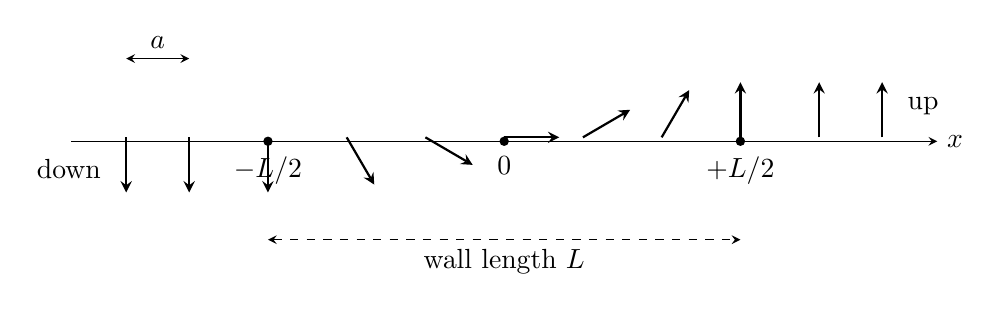
\begin{tikzpicture}[>=stealth, scale=1.0]
  \draw[->] (-5.5,-0.05) -- (5.5,-0.05) node[right] {$x$};
  \node[circle,fill,inner sep=1.2pt,label=below:{$-L/2$}] at (-3,-0.05) {};
  \node[circle,fill,inner sep=1.2pt,label=below:{$0$}]    at ( 0,-0.05) {};
  \node[circle,fill,inner sep=1.2pt,label=below:{$+L/2$}] at ( 3,-0.05) {};
  % spin arrows along the chain (rotate from down to up over [-L/2, +L/2])
  \draw[->,thick] (-4.8,0) -- (-4.8,-0.7);
  \draw[->,thick] (-4.0,0) -- (-4.0,-0.7);
  \draw[->,thick] (-3.0,0) -- (-3.0,-0.7);
  \draw[->,thick] (-2.0,0) -- (-2.0+0.35,-0.6);
  \draw[->,thick] (-1.0,0) -- (-1.0+0.6,-0.35);
  \draw[->,thick] ( 0.0,0) -- ( 0.7,0);
  \draw[->,thick] ( 1.0,0) -- ( 1.0+0.6, 0.35);
  \draw[->,thick] ( 2.0,0) -- ( 2.0+0.35, 0.6);
  \draw[->,thick] ( 3.0,0) -- ( 3.0, 0.7);
  \draw[->,thick] ( 4.0,0) -- ( 4.0, 0.7);
  \draw[->,thick] ( 4.8,0) -- ( 4.8, 0.7);
  \node[left] at (-5.0,-0.4) {down};
  \node[right] at ( 5.0, 0.4) {up};
  \draw[<->,dashed] (-3,-1.3) -- (3,-1.3) node[midway,below] {wall length $L$};
  \draw[<->] (-4.8,1.0) -- (-4.0,1.0) node[midway,above] {$a$};
\end{tikzpicture}
\end{center}

\subsection*{(b) Wall energy as a function of $L$}

Spins rotate uniformly across the wall: take angle from $\hat z$ at site $i$ to be $\theta_i = \pi/2 - \pi x_i/L$. Project onto $\hat z$:
\[
S_i^z = S\cos\theta_i = S\cos(\pi/2 - \pi x_i/L) = S\sin(\pi x_i/L).
\]
Inter-site rotation:
\[
\delta\theta = \theta_{i+1} - \theta_i = -\pi a/L,\qquad |\delta\theta| = \pi a/L.
\]
\textbf{Exchange contribution.} Each bond contributes $-JS^2\cos\delta\theta$. Subtract the uniform-FM bond energy $-JS^2$:
\[
\Delta E_\text{ex,bond} = -JS^2\cos\delta\theta - (-JS^2) = JS^2(1-\cos\delta\theta).
\]
Small-angle expand (since $L\gg a$):
\[
1-\cos\delta\theta \approx \tfrac12(\delta\theta)^2.
\]
Insert $\delta\theta = \pi a/L$:
\[
\Delta E_\text{ex,bond} \approx \tfrac12 JS^2\!\left(\frac{\pi a}{L}\right)^2 = \frac{\pi^2 J S^2 a^2}{2L^2}.
\]
Sum over $L/a$ bonds in the wall:
\[
\Delta E_\text{ex} = \frac{L}{a}\cdot\frac{\pi^2 JS^2 a^2}{2L^2} = \frac{\pi^2 JS^2 a}{2L}.
\]
\textbf{Anisotropy contribution.} Site energy is $-\kappa(S_i^z)^2 = -\kappa S^2\sin^2(\pi x_i/L)$. Subtract uniform $-\kappa S^2$:
\[
\Delta E_\text{an,site} = -\kappa S^2\sin^2(\pi x_i/L) + \kappa S^2 = \kappa S^2(1-\sin^2(\pi x_i/L)).
\]
Apply $\sin^2+\cos^2 = 1$:
\[
\Delta E_\text{an,site} = \kappa S^2 \cos^2(\pi x_i/L).
\]
Convert sum to integral via the hint, $\sum_m f(m\delta)\to (1/\delta)\int f(x)\,\de x$ with $\delta = a$:
\[
\Delta E_\text{an} = \frac{1}{a}\int_{-L/2}^{L/2}\!\kappa S^2 \cos^2(\pi x/L)\,\de x.
\]
Use $\int_{-L/2}^{L/2}\cos^2(\pi x/L)\,\de x = L/2$:
\[
\Delta E_\text{an} = \frac{1}{a}\cdot\kappa S^2\cdot\frac{L}{2} = \frac{\kappa S^2 L}{2a}.
\]
Total wall energy:
\begin{equation}
\boxed{\;\Delta E(L) = \frac{\pi^2 J S^2 a}{2L} + \frac{\kappa S^2 L}{2a}.\;}
\label{eq:dE-L}
\end{equation}

\subsection*{(c) Minimisation}

Differentiate \eqref{eq:dE-L} with respect to $L$:
\[
\frac{\de\,\Delta E}{\de L} = -\frac{\pi^2 JS^2 a}{2L^2} + \frac{\kappa S^2}{2a}.
\]
Set to zero:
\[
\frac{\kappa S^2}{2a} = \frac{\pi^2 JS^2 a}{2L^2}.
\]
Cancel $S^2/2$ on each side:
\[
\frac{\kappa}{a} = \frac{\pi^2 J a}{L^2}.
\]
Solve for $L^2$:
\[
L^2 = \frac{\pi^2 J a^2}{\kappa}.
\]
Take square-root:
\[
\boxed{\;L = \pi\,a\sqrt{J/\kappa},\qquad c_1 = \pi.\;}
\]
Substitute back into the anisotropy term:
\[
\frac{\kappa S^2 L}{2a} = \frac{\kappa S^2}{2a}\cdot\pi a\sqrt{J/\kappa} = \frac{\pi S^2}{2}\cdot\kappa\sqrt{J/\kappa} = \frac{\pi S^2}{2}\sqrt{J\kappa}.
\]
By the symmetry of the optimisation the exchange term equals the anisotropy term:
\[
\Delta E_\text{min} = 2\cdot\frac{\pi S^2}{2}\sqrt{J\kappa} = \pi S^2\sqrt{J\kappa}.
\]
Box:
\[
\boxed{\;\Delta E_\text{min} = \pi S^2\sqrt{J\kappa}.\;}
\]

\subsection*{(d) 2D wall and stripe array}

\textbf{(i) Single wall.} The 2D lattice has $W t/a^2$ parallel chains threading the $y$--$z$ cross-section, each contributing $\Delta E_\text{min}$:
\[
\boxed{\;E_\text{wall} = \frac{Wt}{a^2}\,\pi S^2\sqrt{J\kappa}.\;}
\]

\textbf{(ii) Stripe array.} Walls are spaced $D$ along $x$; the slab volume associated with one wall is $D\cdot W\cdot t$.
\[
\frac{E_\text{walls}}{V_\text{per wall}} = \frac{(Wt/a^2)\,\pi S^2\sqrt{J\kappa}}{D\,W\,t}.
\]
Cancel $Wt$:
\begin{equation}
\boxed{\;\frac{E_\text{walls}}{V} = \frac{\pi S^2\sqrt{J\kappa}}{a^2 D}.\;}
\label{eq:Ewall-vol}
\end{equation}

\subsection*{(e) Equilibrium domain spacing}

Domain walls cost positive exchange + anisotropy energy, but breaking the magnet into alternating-direction stripes lowers the long-range \textbf{magnetostatic (stray-field) energy}, since the surface poles partially cancel between adjacent stripes. Walls form when the magnetostatic saving exceeds the wall cost.

Total energy per unit volume (sum \eqref{eq:Ewall-vol} and the given magnetostatic term):
\[
\frac{E}{V} = \frac{\pi S^2\sqrt{J\kappa}}{a^2 D} + c_2\,\frac{\mu_0 M^2 D}{t}.
\]
Differentiate with respect to $D$ at fixed $t$:
\[
\frac{\de}{\de D}\!\left(\frac{E}{V}\right) = -\frac{\pi S^2\sqrt{J\kappa}}{a^2 D^2} + \frac{c_2\,\mu_0 M^2}{t}.
\]
Set to zero:
\[
\frac{c_2\,\mu_0 M^2}{t} = \frac{\pi S^2\sqrt{J\kappa}}{a^2 D^2}.
\]
Rearrange for $D^2$:
\[
D^2 = \frac{\pi S^2\sqrt{J\kappa}\,t}{c_2\,\mu_0 M^2 a^2}.
\]
Take square-root, so $D\propto\sqrt{t}$:
\[
\boxed{\;D \propto t^{1/2},\qquad \beta = \tfrac12.\;}
\]

\end{document}
